%%%%%%%%%%%%%%%%%%%%%%%%%%%%%%%%%%%%%%%%%
% University Assignment Title Page 
% LaTeX Template
% Version 1.0 (27/12/12)
%
% This template has been downloaded from:
% http://www.LaTeXTemplates.com
%
% Original author:
% WikiBooks (http://en.wikibooks.org/wiki/LaTeX/Title_Creation)
%
% License:
% CC BY-NC-SA 3.0 (http://creativecommons.org/licenses/by-nc-sa/3.0/)
% 
% Instructions for using this template:
% This title page is capable of being compiled as is. This is not useful for 
% including it in another document. To do this, you have two options: 
%
% 1) Copy/paste everything between \begin{document} and \end{document} 
% starting at \begin{titlepage} and paste this into another LaTeX file where you 
% want your title page.
% OR
% 2) Remove everything outside the \begin{titlepage} and \end{titlepage} and 
% move this file to the same directory as the LaTeX file you wish to add it to. 
% Then add %%%%%%%%%%%%%%%%%%%%%%%%%%%%%%%%%%%%%%%%%
% University Assignment Title Page 
% LaTeX Template
% Version 1.0 (27/12/12)
%
% This template has been downloaded from:
% http://www.LaTeXTemplates.com
%
% Original author:
% WikiBooks (http://en.wikibooks.org/wiki/LaTeX/Title_Creation)
%
% License:
% CC BY-NC-SA 3.0 (http://creativecommons.org/licenses/by-nc-sa/3.0/)
% 
% Instructions for using this template:
% This title page is capable of being compiled as is. This is not useful for 
% including it in another document. To do this, you have two options: 
%
% 1) Copy/paste everything between \begin{document} and \end{document} 
% starting at \begin{titlepage} and paste this into another LaTeX file where you 
% want your title page.
% OR
% 2) Remove everything outside the \begin{titlepage} and \end{titlepage} and 
% move this file to the same directory as the LaTeX file you wish to add it to. 
% Then add %%%%%%%%%%%%%%%%%%%%%%%%%%%%%%%%%%%%%%%%%
% University Assignment Title Page 
% LaTeX Template
% Version 1.0 (27/12/12)
%
% This template has been downloaded from:
% http://www.LaTeXTemplates.com
%
% Original author:
% WikiBooks (http://en.wikibooks.org/wiki/LaTeX/Title_Creation)
%
% License:
% CC BY-NC-SA 3.0 (http://creativecommons.org/licenses/by-nc-sa/3.0/)
% 
% Instructions for using this template:
% This title page is capable of being compiled as is. This is not useful for 
% including it in another document. To do this, you have two options: 
%
% 1) Copy/paste everything between \begin{document} and \end{document} 
% starting at \begin{titlepage} and paste this into another LaTeX file where you 
% want your title page.
% OR
% 2) Remove everything outside the \begin{titlepage} and \end{titlepage} and 
% move this file to the same directory as the LaTeX file you wish to add it to. 
% Then add %%%%%%%%%%%%%%%%%%%%%%%%%%%%%%%%%%%%%%%%%
% University Assignment Title Page 
% LaTeX Template
% Version 1.0 (27/12/12)
%
% This template has been downloaded from:
% http://www.LaTeXTemplates.com
%
% Original author:
% WikiBooks (http://en.wikibooks.org/wiki/LaTeX/Title_Creation)
%
% License:
% CC BY-NC-SA 3.0 (http://creativecommons.org/licenses/by-nc-sa/3.0/)
% 
% Instructions for using this template:
% This title page is capable of being compiled as is. This is not useful for 
% including it in another document. To do this, you have two options: 
%
% 1) Copy/paste everything between \begin{document} and \end{document} 
% starting at \begin{titlepage} and paste this into another LaTeX file where you 
% want your title page.
% OR
% 2) Remove everything outside the \begin{titlepage} and \end{titlepage} and 
% move this file to the same directory as the LaTeX file you wish to add it to. 
% Then add \input{./title_page_1.tex} to your LaTeX file where you want your
% title page.
%t
%%%%%%%%%%%%%%%%%%%%%%%%%%%%%%%%%%%%%%%%%
\title{Neo4j cơ bản và ứng dụng}
%----------------------------------------------------------------------------------------
%	PACKAGES AND OTHER DOCUMENT CONFIGURATIONS
%----------------------------------------------------------------------------------------

\documentclass[12pt]{article}
\usepackage[T5]{fontenc}
\usepackage[utf8]{inputenc}
\usepackage[vietnamese,english]{babel}
\usepackage{amsmath}
\usepackage{graphicx}
\usepackage[colorinlistoftodos]{todonotes}

\usepackage{hyperref}
\hypersetup{
    colorlinks=true,
    linkcolor=blue,
    filecolor=magenta,      
    urlcolor=cyan,
}


\begin{document}

\begin{titlepage}

\newcommand{\HRule}{\rule{\linewidth}{0.5mm}} % Defines a new command for the horizontal lines, change thickness here

\center % Center everything on the page
 
%----------------------------------------------------------------------------------------
%	HEADING SECTIONS
%----------------------------------------------------------------------------------------

\textsc{\LARGE Đại học Khoa học tự nhiên}\\[1.5cm] % Name of your university/college
\textsc{\Large Ngành hệ thống thông tin}\\[0.5cm] % Major heading such as course name
\textsc{\large Môn học: Cơ sở dữ liệu nâng cao}\\[0.5cm] % Minor heading such as course title

%----------------------------------------------------------------------------------------
%	TITLE SECTION
%----------------------------------------------------------------------------------------

\HRule \\[0.4cm]
{ \huge \bfseries Neo4j cơ bản và ứng dụng}\\[0.4cm] % Title of your document
\HRule \\[1.5cm]
 
%----------------------------------------------------------------------------------------
%	AUTHOR SECTION
%----------------------------------------------------------------------------------------

\begin{minipage}{0.4\textwidth}
\begin{flushleft} \large
\emph{Học viên:}\\
Thái Thiện -- 17C 12 031 % Your name
\end{flushleft}
\end{minipage}
~
\begin{minipage}{0.4\textwidth}
\begin{flushright} \large
\emph{Giảng viên:} \\
TS. Nguyễn Trần Minh Thư % Supervisor's Name
\end{flushright}
\end{minipage}\\[2cm]

% If you don't want a supervisor, uncomment the two lines below and remove the section above
%\Large \emph{Author:}\\
%John \textsc{Smith}\\[3cm] % Your name

%----------------------------------------------------------------------------------------
%	DATE SECTION
%----------------------------------------------------------------------------------------

% I don't want day because it is English
% {\large \today}\\[2cm] % Date, change the \today to a set date if you want to be precise

%----------------------------------------------------------------------------------------
%	LOGO SECTION
%----------------------------------------------------------------------------------------


\includegraphics{logo/rsz_3logo-khtn.png}\\[1cm] % Include a department/university logo - this will require the graphicx package
 
%----------------------------------------------------------------------------------------

\vfill % Fill the rest of the page with whitespace

\end{titlepage}


\section{Giới thiệu}
Neo4j là nền tảng cơ sở dữ liệu đồ thị (Neo4j Graph Platform) được công ty Neo4j phát triển. 

Trang chủ:  \url{https://neo4j.com}   
% \section{Some \LaTeX{} Examples}
% \label{sec:examples}

\subsection{Các phiên bản}
Neo4j có 2 phiên bản \footnote{\url{https://neo4j.com/subscriptions/}}

\begin{itemize}
\item \textbf{Community Edition} - Phiên bản cộng đồng: Đây là phiên bản miễn phí mã nguồn mở. Thích hợp cho các dự án nhỏ.
\item \textbf{Enterprise Edition} - Phiên bản doanh nghiệp: hiên bản có phí cho doanh nghiệp, có thêm nhiều chức năng như khả năng mở rộng theo chiều dài và chiều sâu, chức năng quản lý phân quyền. Ngoài ra, hiệu suất của phiên bản doanh nghiệp cao hơn phiên bản cộng đồng (vd: câu truy vấn nhanh hơn 70\%, ghi dữ liệu nhanh gấp 5 lần). Phiên bản doanh nghiệp bao gồm hỗ trợ kỹ thuật từ Neo4j 
\end{itemize}

\subsection{Cài đặt}
Tài về:  \url{https://neo4j.com/download/}  
Có thể cài bảng Neo4j Desktop trên máy tính cá nhân. 


\section{Cơ sở dữ liệu đồ thị}
Neo4j sử dụng Mô hình biểu đồ thuộc tính được gắn nhãn (Labeled Property Graph Mode). 

Mô hình bao gồm 4 thành phần: 

\begin{itemize}
\item Nút (nodes)
\item Quan hệ (relationships)
\item Thuộc tính  (properties)
\item Nhãn (labels)
\end{itemize}

\subsection{Nút (nodes)}
Nút (nodes) chứa các thuộc tính (properties). Một nút có thể xem là một bảng ghi gồm nhiều các cặp khóa - giá trị tùy ý. Trong Neo4j, khóa là chuổi còn giá trị là chuỗi Java và các kiểu dữ liệu nguyên thủy, và mảng của các dữ liệu đó. 

% % Commands to include a figure:
\begin{figure}[h]
\centering
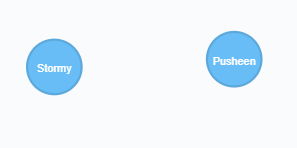
\includegraphics[width=0.5\textwidth]{image/node.PNG}
\caption{\label{fig:node} Nút}
\end{figure}

\begin{figure}[h]
\centering
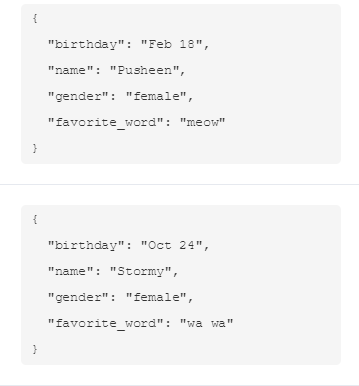
\includegraphics[width=0.5\textwidth]{image/thuoc_tinh.PNG}
\caption{\label{fig:node} Thuộc tính của nút}
\end{figure}

Mỗi nút có thể chứa 1 (hoặc nhiều) nhãn (labels). Nhãn giúp nhóm các nút lại với nhau. Có thể hiểu nhãn của nút là loại thực thể (mèo, đồ ăn, ...) của nút đó. Ví dụ hình \ref{fig:catfoodnode}, Nút xanh gán nhãn mèo, còn nút đỏ gán nhãn thức ăn.

\begin{figure}[h]
\centering
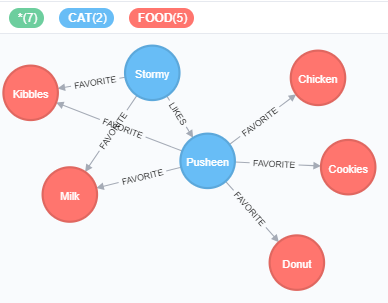
\includegraphics[width=0.5\textwidth]{image/complete_node_with_cat_and_food.PNG}
\caption{\label{fig:catfoodnode} Nút mèo và nút thức ăn}
\end{figure}

\subsection{Quan hệ (relationships)}
Quan hệ nối các nút lại để tạo thành biểu đồ. Mỗi quan hệ luôn có: 

\begin{itemize}
\item Tên quan hệ
\item Hướng 
\item Nút đầu
\item Nút cuối
\end{itemize}

Hình \ref{fig:relationships} biểu diễn quan hệ LIKES từ nút CAT có name = "Stormy" đến nút CAT có name = "Pusheen"

\begin{figure}[h]
\centering
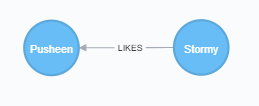
\includegraphics[width=0.5\textwidth]{image/relationships.PNG}
\caption{\label{fig:relationships} Quan hệ LIKES từ mèo Stormy đối với Pusheen}
\end{figure}

Quan hệ có thể chứa thuộc tính (properties) như nút (hình \ref{fig:relationshipsprop}). 

\begin{figure}[h]
\centering
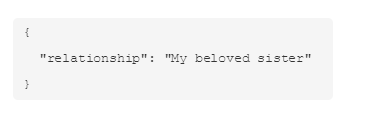
\includegraphics[width=0.5\textwidth]{image/quan_he_thuoc_tin.PNG}
\caption{\label{fig:relationshipsprop} Quan hệ LIKES từ mèo Stormy đối với Pusheen}
\end{figure}


\section{Cypher}



Comments can be added to the margins of the document using the \todo{Here's a comment in the margin!} todo command, as shown in the example on the right. You can also add inline comments too:

\todo[inline, color=green!40]{This is an inline comment.}

\subsection{Tables and Figures}

Use the table and tabular commands for basic tables --- see Table~\ref{tab:widgets}, for example. You can upload a figure (JPEG, PNG or PDF) using the files menu. To include it in your document, use the includegraphics command as in the code for Figure~\ref{fig:frog} below.

% % Commands to include a figure:
% \begin{figure}
% \centering
% 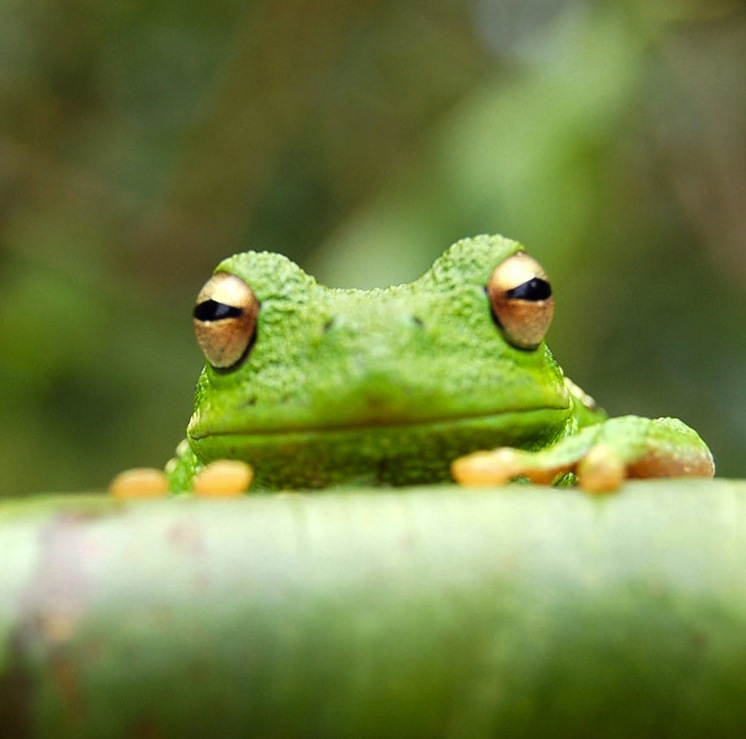
\includegraphics[width=0.5\textwidth]{frog.jpg}
% \caption{\label{fig:frog}This is a figure caption.}
% \end{figure}

% \begin{table}
% \centering
% \begin{tabular}{l|r}
% Item & Quantity \\\hline
% Widgets & 42 \\
% Gadgets & 13
% \end{tabular}
% \caption{\label{tab:widgets}An example table.}
% \end{table}

\subsection{Mathematics}

\LaTeX{} is great at typesetting mathematics. Let $X_1, X_2, \ldots, X_n$ be a sequence of independent and identically distributed random variables with $\text{E}[X_i] = \mu$ and $\text{Var}[X_i] = \sigma^2 < \infty$, and let
$$S_n = \frac{X_1 + X_2 + \cdots + X_n}{n}
      = \frac{1}{n}\sum_{i}^{n} X_i$$
denote their mean. Then as $n$ approaches infinity, the random variables $\sqrt{n}(S_n - \mu)$ converge in distribution to a normal $\mathcal{N}(0, \sigma^2)$.

\subsection{Lists}

You can make lists with automatic numbering \dots

\begin{enumerate}
\item Like this,
\item and like this.
\end{enumerate}
\dots or bullet points \dots
\begin{itemize}
\item Like this,
\item and like this.
\end{itemize}

We hope you find write\LaTeX\ useful, and please let us know if you have any feedback using the help menu above.

\end{document} to your LaTeX file where you want your
% title page.
%t
%%%%%%%%%%%%%%%%%%%%%%%%%%%%%%%%%%%%%%%%%
\title{Neo4j cơ bản và ứng dụng}
%----------------------------------------------------------------------------------------
%	PACKAGES AND OTHER DOCUMENT CONFIGURATIONS
%----------------------------------------------------------------------------------------

\documentclass[12pt]{article}
\usepackage[T5]{fontenc}
\usepackage[utf8]{inputenc}
\usepackage[vietnamese,english]{babel}
\usepackage{amsmath}
\usepackage{graphicx}
\usepackage[colorinlistoftodos]{todonotes}

\usepackage{hyperref}
\hypersetup{
    colorlinks=true,
    linkcolor=blue,
    filecolor=magenta,      
    urlcolor=cyan,
}


\begin{document}

\begin{titlepage}

\newcommand{\HRule}{\rule{\linewidth}{0.5mm}} % Defines a new command for the horizontal lines, change thickness here

\center % Center everything on the page
 
%----------------------------------------------------------------------------------------
%	HEADING SECTIONS
%----------------------------------------------------------------------------------------

\textsc{\LARGE Đại học Khoa học tự nhiên}\\[1.5cm] % Name of your university/college
\textsc{\Large Ngành hệ thống thông tin}\\[0.5cm] % Major heading such as course name
\textsc{\large Môn học: Cơ sở dữ liệu nâng cao}\\[0.5cm] % Minor heading such as course title

%----------------------------------------------------------------------------------------
%	TITLE SECTION
%----------------------------------------------------------------------------------------

\HRule \\[0.4cm]
{ \huge \bfseries Neo4j cơ bản và ứng dụng}\\[0.4cm] % Title of your document
\HRule \\[1.5cm]
 
%----------------------------------------------------------------------------------------
%	AUTHOR SECTION
%----------------------------------------------------------------------------------------

\begin{minipage}{0.4\textwidth}
\begin{flushleft} \large
\emph{Học viên:}\\
Thái Thiện -- 17C 12 031 % Your name
\end{flushleft}
\end{minipage}
~
\begin{minipage}{0.4\textwidth}
\begin{flushright} \large
\emph{Giảng viên:} \\
TS. Nguyễn Trần Minh Thư % Supervisor's Name
\end{flushright}
\end{minipage}\\[2cm]

% If you don't want a supervisor, uncomment the two lines below and remove the section above
%\Large \emph{Author:}\\
%John \textsc{Smith}\\[3cm] % Your name

%----------------------------------------------------------------------------------------
%	DATE SECTION
%----------------------------------------------------------------------------------------

% I don't want day because it is English
% {\large \today}\\[2cm] % Date, change the \today to a set date if you want to be precise

%----------------------------------------------------------------------------------------
%	LOGO SECTION
%----------------------------------------------------------------------------------------


\includegraphics{logo/rsz_3logo-khtn.png}\\[1cm] % Include a department/university logo - this will require the graphicx package
 
%----------------------------------------------------------------------------------------

\vfill % Fill the rest of the page with whitespace

\end{titlepage}


\section{Giới thiệu}
Neo4j là nền tảng cơ sở dữ liệu đồ thị (Neo4j Graph Platform) được công ty Neo4j phát triển. 

Trang chủ:  \url{https://neo4j.com}   
% \section{Some \LaTeX{} Examples}
% \label{sec:examples}

\subsection{Các phiên bản}
Neo4j có 2 phiên bản \footnote{\url{https://neo4j.com/subscriptions/}}

\begin{itemize}
\item \textbf{Community Edition} - Phiên bản cộng đồng: Đây là phiên bản miễn phí mã nguồn mở. Thích hợp cho các dự án nhỏ.
\item \textbf{Enterprise Edition} - Phiên bản doanh nghiệp: hiên bản có phí cho doanh nghiệp, có thêm nhiều chức năng như khả năng mở rộng theo chiều dài và chiều sâu, chức năng quản lý phân quyền. Ngoài ra, hiệu suất của phiên bản doanh nghiệp cao hơn phiên bản cộng đồng (vd: câu truy vấn nhanh hơn 70\%, ghi dữ liệu nhanh gấp 5 lần). Phiên bản doanh nghiệp bao gồm hỗ trợ kỹ thuật từ Neo4j 
\end{itemize}

\subsection{Cài đặt}
Tài về:  \url{https://neo4j.com/download/}  
Có thể cài bảng Neo4j Desktop trên máy tính cá nhân. 


\section{Cơ sở dữ liệu đồ thị}
Neo4j sử dụng Mô hình biểu đồ thuộc tính được gắn nhãn (Labeled Property Graph Mode). 

Mô hình bao gồm 4 thành phần: 

\begin{itemize}
\item Nút (nodes)
\item Quan hệ (relationships)
\item Thuộc tính  (properties)
\item Nhãn (labels)
\end{itemize}

\subsection{Nút (nodes)}
Nút (nodes) chứa các thuộc tính (properties). Một nút có thể xem là một bảng ghi gồm nhiều các cặp khóa - giá trị tùy ý. Trong Neo4j, khóa là chuổi còn giá trị là chuỗi Java và các kiểu dữ liệu nguyên thủy, và mảng của các dữ liệu đó. 

% % Commands to include a figure:
\begin{figure}[h]
\centering
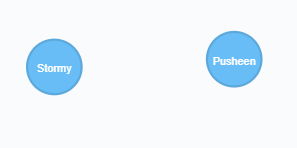
\includegraphics[width=0.5\textwidth]{image/node.PNG}
\caption{\label{fig:node} Nút}
\end{figure}

\begin{figure}[h]
\centering
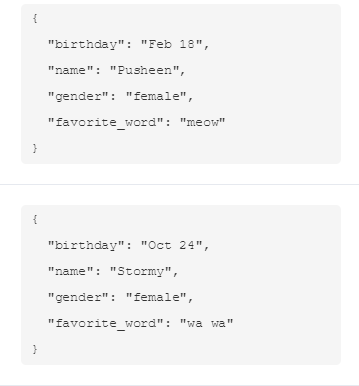
\includegraphics[width=0.5\textwidth]{image/thuoc_tinh.PNG}
\caption{\label{fig:node} Thuộc tính của nút}
\end{figure}

Mỗi nút có thể chứa 1 (hoặc nhiều) nhãn (labels). Nhãn giúp nhóm các nút lại với nhau. Có thể hiểu nhãn của nút là loại thực thể (mèo, đồ ăn, ...) của nút đó. Ví dụ hình \ref{fig:catfoodnode}, Nút xanh gán nhãn mèo, còn nút đỏ gán nhãn thức ăn.

\begin{figure}[h]
\centering
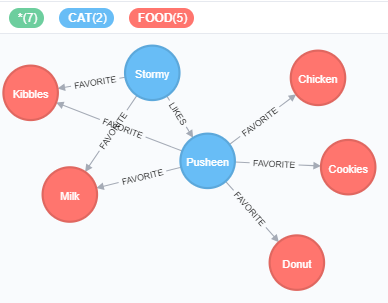
\includegraphics[width=0.5\textwidth]{image/complete_node_with_cat_and_food.PNG}
\caption{\label{fig:catfoodnode} Nút mèo và nút thức ăn}
\end{figure}

\subsection{Quan hệ (relationships)}
Quan hệ nối các nút lại để tạo thành biểu đồ. Mỗi quan hệ luôn có: 

\begin{itemize}
\item Tên quan hệ
\item Hướng 
\item Nút đầu
\item Nút cuối
\end{itemize}

Hình \ref{fig:relationships} biểu diễn quan hệ LIKES từ nút CAT có name = "Stormy" đến nút CAT có name = "Pusheen"

\begin{figure}[h]
\centering
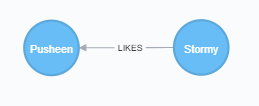
\includegraphics[width=0.5\textwidth]{image/relationships.PNG}
\caption{\label{fig:relationships} Quan hệ LIKES từ mèo Stormy đối với Pusheen}
\end{figure}

Quan hệ có thể chứa thuộc tính (properties) như nút (hình \ref{fig:relationshipsprop}). 

\begin{figure}[h]
\centering
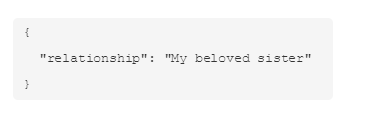
\includegraphics[width=0.5\textwidth]{image/quan_he_thuoc_tin.PNG}
\caption{\label{fig:relationshipsprop} Quan hệ LIKES từ mèo Stormy đối với Pusheen}
\end{figure}


\section{Cypher}



Comments can be added to the margins of the document using the \todo{Here's a comment in the margin!} todo command, as shown in the example on the right. You can also add inline comments too:

\todo[inline, color=green!40]{This is an inline comment.}

\subsection{Tables and Figures}

Use the table and tabular commands for basic tables --- see Table~\ref{tab:widgets}, for example. You can upload a figure (JPEG, PNG or PDF) using the files menu. To include it in your document, use the includegraphics command as in the code for Figure~\ref{fig:frog} below.

% % Commands to include a figure:
% \begin{figure}
% \centering
% 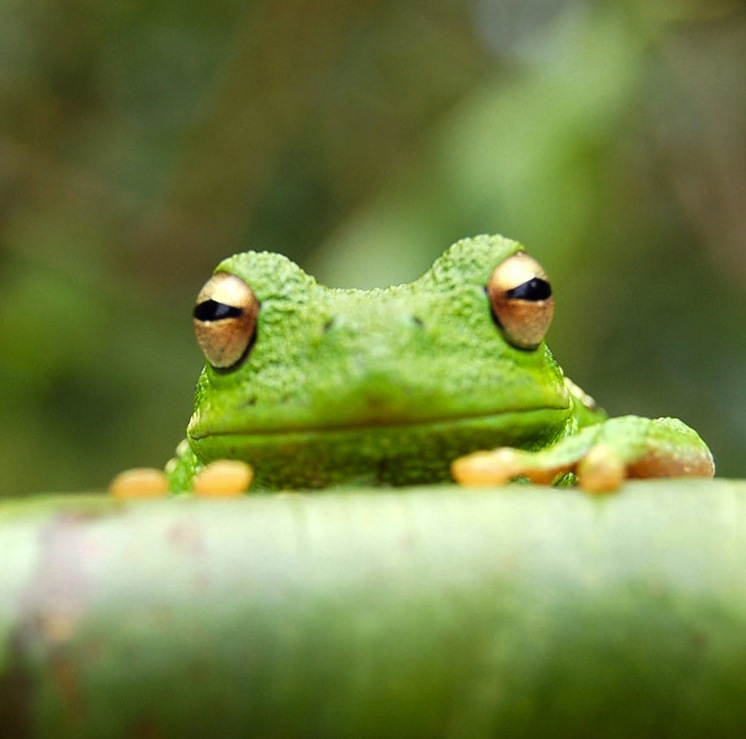
\includegraphics[width=0.5\textwidth]{frog.jpg}
% \caption{\label{fig:frog}This is a figure caption.}
% \end{figure}

% \begin{table}
% \centering
% \begin{tabular}{l|r}
% Item & Quantity \\\hline
% Widgets & 42 \\
% Gadgets & 13
% \end{tabular}
% \caption{\label{tab:widgets}An example table.}
% \end{table}

\subsection{Mathematics}

\LaTeX{} is great at typesetting mathematics. Let $X_1, X_2, \ldots, X_n$ be a sequence of independent and identically distributed random variables with $\text{E}[X_i] = \mu$ and $\text{Var}[X_i] = \sigma^2 < \infty$, and let
$$S_n = \frac{X_1 + X_2 + \cdots + X_n}{n}
      = \frac{1}{n}\sum_{i}^{n} X_i$$
denote their mean. Then as $n$ approaches infinity, the random variables $\sqrt{n}(S_n - \mu)$ converge in distribution to a normal $\mathcal{N}(0, \sigma^2)$.

\subsection{Lists}

You can make lists with automatic numbering \dots

\begin{enumerate}
\item Like this,
\item and like this.
\end{enumerate}
\dots or bullet points \dots
\begin{itemize}
\item Like this,
\item and like this.
\end{itemize}

We hope you find write\LaTeX\ useful, and please let us know if you have any feedback using the help menu above.

\end{document} to your LaTeX file where you want your
% title page.
%t
%%%%%%%%%%%%%%%%%%%%%%%%%%%%%%%%%%%%%%%%%
\title{Neo4j cơ bản và ứng dụng}
%----------------------------------------------------------------------------------------
%	PACKAGES AND OTHER DOCUMENT CONFIGURATIONS
%----------------------------------------------------------------------------------------

\documentclass[12pt]{article}
\usepackage[T5]{fontenc}
\usepackage[utf8]{inputenc}
\usepackage[vietnamese,english]{babel}
\usepackage{amsmath}
\usepackage{graphicx}
\usepackage[colorinlistoftodos]{todonotes}

\usepackage{hyperref}
\hypersetup{
    colorlinks=true,
    linkcolor=blue,
    filecolor=magenta,      
    urlcolor=cyan,
}


\begin{document}

\begin{titlepage}

\newcommand{\HRule}{\rule{\linewidth}{0.5mm}} % Defines a new command for the horizontal lines, change thickness here

\center % Center everything on the page
 
%----------------------------------------------------------------------------------------
%	HEADING SECTIONS
%----------------------------------------------------------------------------------------

\textsc{\LARGE Đại học Khoa học tự nhiên}\\[1.5cm] % Name of your university/college
\textsc{\Large Ngành hệ thống thông tin}\\[0.5cm] % Major heading such as course name
\textsc{\large Môn học: Cơ sở dữ liệu nâng cao}\\[0.5cm] % Minor heading such as course title

%----------------------------------------------------------------------------------------
%	TITLE SECTION
%----------------------------------------------------------------------------------------

\HRule \\[0.4cm]
{ \huge \bfseries Neo4j cơ bản và ứng dụng}\\[0.4cm] % Title of your document
\HRule \\[1.5cm]
 
%----------------------------------------------------------------------------------------
%	AUTHOR SECTION
%----------------------------------------------------------------------------------------

\begin{minipage}{0.4\textwidth}
\begin{flushleft} \large
\emph{Học viên:}\\
Thái Thiện -- 17C 12 031 % Your name
\end{flushleft}
\end{minipage}
~
\begin{minipage}{0.4\textwidth}
\begin{flushright} \large
\emph{Giảng viên:} \\
TS. Nguyễn Trần Minh Thư % Supervisor's Name
\end{flushright}
\end{minipage}\\[2cm]

% If you don't want a supervisor, uncomment the two lines below and remove the section above
%\Large \emph{Author:}\\
%John \textsc{Smith}\\[3cm] % Your name

%----------------------------------------------------------------------------------------
%	DATE SECTION
%----------------------------------------------------------------------------------------

% I don't want day because it is English
% {\large \today}\\[2cm] % Date, change the \today to a set date if you want to be precise

%----------------------------------------------------------------------------------------
%	LOGO SECTION
%----------------------------------------------------------------------------------------


\includegraphics{logo/rsz_3logo-khtn.png}\\[1cm] % Include a department/university logo - this will require the graphicx package
 
%----------------------------------------------------------------------------------------

\vfill % Fill the rest of the page with whitespace

\end{titlepage}


\section{Giới thiệu}
Neo4j là nền tảng cơ sở dữ liệu đồ thị (Neo4j Graph Platform) được công ty Neo4j phát triển. 

Trang chủ:  \url{https://neo4j.com}   
% \section{Some \LaTeX{} Examples}
% \label{sec:examples}

\subsection{Các phiên bản}
Neo4j có 2 phiên bản \footnote{\url{https://neo4j.com/subscriptions/}}

\begin{itemize}
\item \textbf{Community Edition} - Phiên bản cộng đồng: Đây là phiên bản miễn phí mã nguồn mở. Thích hợp cho các dự án nhỏ.
\item \textbf{Enterprise Edition} - Phiên bản doanh nghiệp: hiên bản có phí cho doanh nghiệp, có thêm nhiều chức năng như khả năng mở rộng theo chiều dài và chiều sâu, chức năng quản lý phân quyền. Ngoài ra, hiệu suất của phiên bản doanh nghiệp cao hơn phiên bản cộng đồng (vd: câu truy vấn nhanh hơn 70\%, ghi dữ liệu nhanh gấp 5 lần). Phiên bản doanh nghiệp bao gồm hỗ trợ kỹ thuật từ Neo4j 
\end{itemize}

\subsection{Cài đặt}
Tài về:  \url{https://neo4j.com/download/}  
Có thể cài bảng Neo4j Desktop trên máy tính cá nhân. 


\section{Cơ sở dữ liệu đồ thị}
Neo4j sử dụng Mô hình biểu đồ thuộc tính được gắn nhãn (Labeled Property Graph Mode). 

Mô hình bao gồm 4 thành phần: 

\begin{itemize}
\item Nút (nodes)
\item Quan hệ (relationships)
\item Thuộc tính  (properties)
\item Nhãn (labels)
\end{itemize}

\subsection{Nút (nodes)}
Nút (nodes) chứa các thuộc tính (properties). Một nút có thể xem là một bảng ghi gồm nhiều các cặp khóa - giá trị tùy ý. Trong Neo4j, khóa là chuổi còn giá trị là chuỗi Java và các kiểu dữ liệu nguyên thủy, và mảng của các dữ liệu đó. 

% % Commands to include a figure:
\begin{figure}[h]
\centering
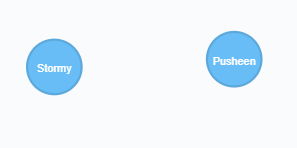
\includegraphics[width=0.5\textwidth]{image/node.PNG}
\caption{\label{fig:node} Nút}
\end{figure}

\begin{figure}[h]
\centering
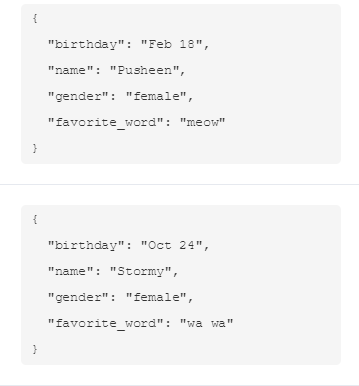
\includegraphics[width=0.5\textwidth]{image/thuoc_tinh.PNG}
\caption{\label{fig:node} Thuộc tính của nút}
\end{figure}

Mỗi nút có thể chứa 1 (hoặc nhiều) nhãn (labels). Nhãn giúp nhóm các nút lại với nhau. Có thể hiểu nhãn của nút là loại thực thể (mèo, đồ ăn, ...) của nút đó. Ví dụ hình \ref{fig:catfoodnode}, Nút xanh gán nhãn mèo, còn nút đỏ gán nhãn thức ăn.

\begin{figure}[h]
\centering
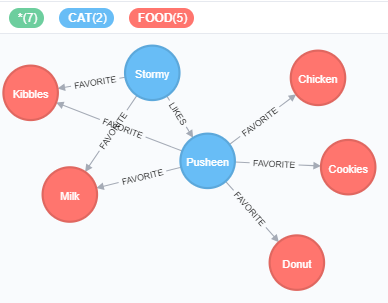
\includegraphics[width=0.5\textwidth]{image/complete_node_with_cat_and_food.PNG}
\caption{\label{fig:catfoodnode} Nút mèo và nút thức ăn}
\end{figure}

\subsection{Quan hệ (relationships)}
Quan hệ nối các nút lại để tạo thành biểu đồ. Mỗi quan hệ luôn có: 

\begin{itemize}
\item Tên quan hệ
\item Hướng 
\item Nút đầu
\item Nút cuối
\end{itemize}

Hình \ref{fig:relationships} biểu diễn quan hệ LIKES từ nút CAT có name = "Stormy" đến nút CAT có name = "Pusheen"

\begin{figure}[h]
\centering
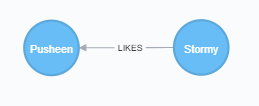
\includegraphics[width=0.5\textwidth]{image/relationships.PNG}
\caption{\label{fig:relationships} Quan hệ LIKES từ mèo Stormy đối với Pusheen}
\end{figure}

Quan hệ có thể chứa thuộc tính (properties) như nút (hình \ref{fig:relationshipsprop}). 

\begin{figure}[h]
\centering
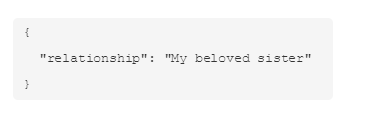
\includegraphics[width=0.5\textwidth]{image/quan_he_thuoc_tin.PNG}
\caption{\label{fig:relationshipsprop} Quan hệ LIKES từ mèo Stormy đối với Pusheen}
\end{figure}


\section{Cypher}



Comments can be added to the margins of the document using the \todo{Here's a comment in the margin!} todo command, as shown in the example on the right. You can also add inline comments too:

\todo[inline, color=green!40]{This is an inline comment.}

\subsection{Tables and Figures}

Use the table and tabular commands for basic tables --- see Table~\ref{tab:widgets}, for example. You can upload a figure (JPEG, PNG or PDF) using the files menu. To include it in your document, use the includegraphics command as in the code for Figure~\ref{fig:frog} below.

% % Commands to include a figure:
% \begin{figure}
% \centering
% 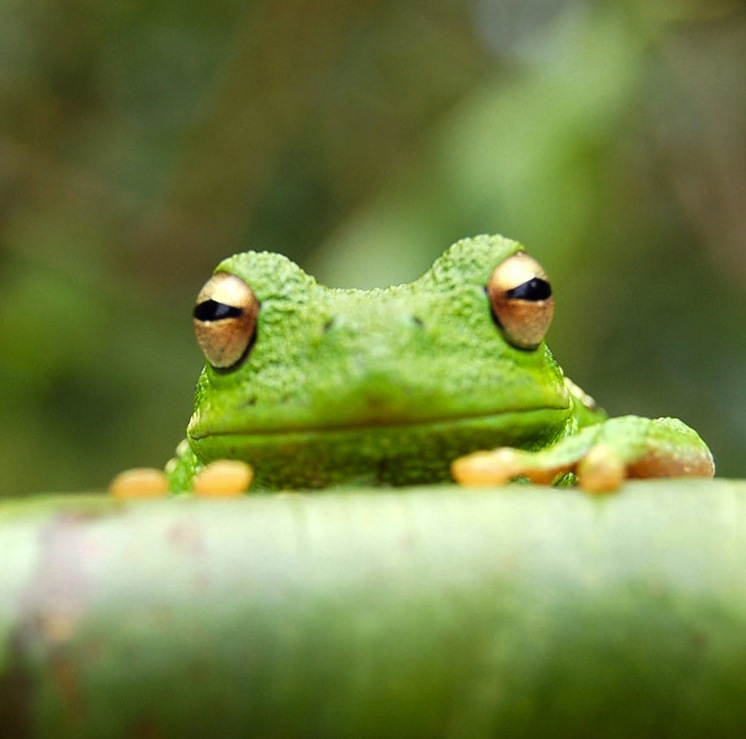
\includegraphics[width=0.5\textwidth]{frog.jpg}
% \caption{\label{fig:frog}This is a figure caption.}
% \end{figure}

% \begin{table}
% \centering
% \begin{tabular}{l|r}
% Item & Quantity \\\hline
% Widgets & 42 \\
% Gadgets & 13
% \end{tabular}
% \caption{\label{tab:widgets}An example table.}
% \end{table}

\subsection{Mathematics}

\LaTeX{} is great at typesetting mathematics. Let $X_1, X_2, \ldots, X_n$ be a sequence of independent and identically distributed random variables with $\text{E}[X_i] = \mu$ and $\text{Var}[X_i] = \sigma^2 < \infty$, and let
$$S_n = \frac{X_1 + X_2 + \cdots + X_n}{n}
      = \frac{1}{n}\sum_{i}^{n} X_i$$
denote their mean. Then as $n$ approaches infinity, the random variables $\sqrt{n}(S_n - \mu)$ converge in distribution to a normal $\mathcal{N}(0, \sigma^2)$.

\subsection{Lists}

You can make lists with automatic numbering \dots

\begin{enumerate}
\item Like this,
\item and like this.
\end{enumerate}
\dots or bullet points \dots
\begin{itemize}
\item Like this,
\item and like this.
\end{itemize}

We hope you find write\LaTeX\ useful, and please let us know if you have any feedback using the help menu above.

\end{document} to your LaTeX file where you want your
% title page.
%t
%%%%%%%%%%%%%%%%%%%%%%%%%%%%%%%%%%%%%%%%%
\title{Neo4j cơ bản và ứng dụng}
%----------------------------------------------------------------------------------------
%	PACKAGES AND OTHER DOCUMENT CONFIGURATIONS
%----------------------------------------------------------------------------------------

\documentclass[12pt]{article}
\usepackage[T5]{fontenc}
\usepackage[utf8]{inputenc}
\usepackage[vietnamese,english]{babel}
\usepackage{amsmath}
\usepackage{graphicx}
\usepackage[colorinlistoftodos]{todonotes}
\usepackage{listings}
\usepackage{hyperref}
\hypersetup{
    colorlinks=true,
    linkcolor=blue,
    filecolor=magenta,      
    urlcolor=cyan,
}


\begin{document}

\begin{titlepage}

\newcommand{\HRule}{\rule{\linewidth}{0.5mm}} % Defines a new command for the horizontal lines, change thickness here

\center % Center everything on the page
 
%----------------------------------------------------------------------------------------
%	HEADING SECTIONS
%----------------------------------------------------------------------------------------

\textsc{\LARGE Đại học Khoa học tự nhiên}\\[1.5cm] % Name of your university/college
\textsc{\Large Ngành hệ thống thông tin}\\[0.5cm] % Major heading such as course name
\textsc{\large Môn học: Cơ sở dữ liệu nâng cao}\\[0.5cm] % Minor heading such as course title

%----------------------------------------------------------------------------------------
%	TITLE SECTION
%----------------------------------------------------------------------------------------

\HRule \\[0.4cm]
{ \huge \bfseries Neo4j cơ bản và ứng dụng}\\[0.4cm] % Title of your document
\HRule \\[1.5cm]
 
%----------------------------------------------------------------------------------------
%	AUTHOR SECTION
%----------------------------------------------------------------------------------------

\begin{minipage}{0.4\textwidth}
\begin{flushleft} \large
\emph{Học viên:}\\
Thái Thiện -- 17C 12 031 % Your name
\end{flushleft}
\end{minipage}
~
\begin{minipage}{0.4\textwidth}
\begin{flushright} \large
\emph{Giảng viên:} \\
TS. Nguyễn Trần Minh Thư % Supervisor's Name
\end{flushright}
\end{minipage}\\[2cm]

% If you don't want a supervisor, uncomment the two lines below and remove the section above
%\Large \emph{Author:}\\
%John \textsc{Smith}\\[3cm] % Your name

%----------------------------------------------------------------------------------------
%	DATE SECTION
%----------------------------------------------------------------------------------------

% I don't want day because it is English
% {\large \today}\\[2cm] % Date, change the \today to a set date if you want to be precise

%----------------------------------------------------------------------------------------
%	LOGO SECTION
%----------------------------------------------------------------------------------------


\includegraphics{logo/rsz_3logo-khtn.png}\\[1cm] % Include a department/university logo - this will require the graphicx package
 
%----------------------------------------------------------------------------------------

\vfill % Fill the rest of the page with whitespace

\end{titlepage}


\section{Giới thiệu}
Neo4j là nền tảng cơ sở dữ liệu đồ thị (Neo4j Graph Platform) được công ty Neo4j phát triển. 

Trang chủ:  \url{https://neo4j.com}   
% \section{Some \LaTeX{} Examples}
% \label{sec:examples}

\subsection{Các phiên bản}
Neo4j có 2 phiên bản \footnote{\url{https://neo4j.com/subscriptions/}}

\begin{itemize}
\item \textbf{Community Edition} - Phiên bản cộng đồng: Đây là phiên bản miễn phí mã nguồn mở. Thích hợp cho các dự án nhỏ.
\item \textbf{Enterprise Edition} - Phiên bản doanh nghiệp: hiên bản có phí cho doanh nghiệp, có thêm nhiều chức năng như khả năng mở rộng theo chiều dài và chiều sâu, chức năng quản lý phân quyền. Ngoài ra, hiệu suất của phiên bản doanh nghiệp cao hơn phiên bản cộng đồng (vd: câu truy vấn nhanh hơn 70\%, ghi dữ liệu nhanh gấp 5 lần). Phiên bản doanh nghiệp bao gồm hỗ trợ kỹ thuật từ Neo4j 
\end{itemize}

\subsection{Cài đặt}
Tài về:  \url{https://neo4j.com/download/}  
Có thể cài bảng Neo4j Desktop trên máy tính cá nhân. 


\section{Cơ sở dữ liệu đồ thị}
Neo4j sử dụng Mô hình biểu đồ thuộc tính được gắn nhãn (Labeled Property Graph Mode). 

Mô hình bao gồm 4 thành phần: 

\begin{itemize}
\item Nút (nodes)
\item Quan hệ (relationships)
\item Thuộc tính  (properties)
\item Nhãn (labels)
\end{itemize}

\subsection{Nút (nodes)}
Nút (nodes) chứa các thuộc tính (properties). Một nút có thể xem là một bảng ghi gồm nhiều các cặp khóa - giá trị tùy ý. Trong Neo4j, khóa là chuổi còn giá trị là chuỗi Java và các kiểu dữ liệu nguyên thủy, và mảng của các dữ liệu đó. 

% % Commands to include a figure:
\begin{figure}[h]
\centering
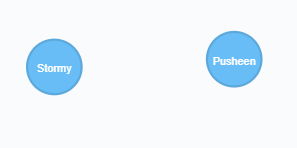
\includegraphics[width=0.5\textwidth]{image/node.PNG}
\caption{\label{fig:node} Nút}
\end{figure}

\begin{figure}[h]
\centering
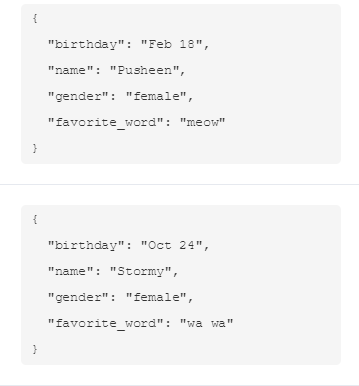
\includegraphics[width=0.5\textwidth]{image/thuoc_tinh.PNG}
\caption{\label{fig:node} Thuộc tính của nút}
\end{figure}

Mỗi nút có thể chứa 1 (hoặc nhiều) nhãn (labels). Nhãn giúp nhóm các nút lại với nhau. Có thể hiểu nhãn của nút là loại thực thể (mèo, đồ ăn, ...) của nút đó. Ví dụ hình \ref{fig:catfoodnode}, Nút xanh gán nhãn mèo, còn nút đỏ gán nhãn thức ăn.

\begin{figure}[h]
\centering
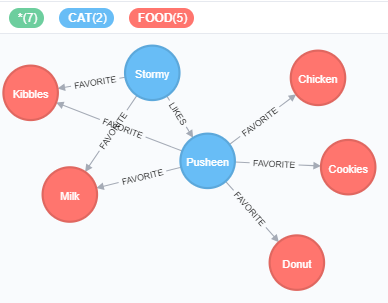
\includegraphics[width=0.5\textwidth]{image/complete_node_with_cat_and_food.PNG}
\caption{\label{fig:catfoodnode} Nút mèo và nút thức ăn}
\end{figure}

\subsection{Quan hệ (relationships)}
Quan hệ nối các nút lại để tạo thành biểu đồ. Mỗi quan hệ luôn có: 

\begin{itemize}
\item Tên quan hệ
\item Hướng 
\item Nút đầu
\item Nút cuối
\end{itemize}

Hình \ref{fig:relationships} biểu diễn quan hệ LIKES từ nút CAT có name = "Stormy" đến nút CAT có name = "Pusheen"

\begin{figure}[h]
\centering
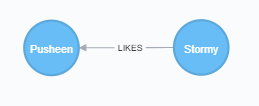
\includegraphics[width=0.7\textwidth]{image/relationships.PNG}
\caption{\label{fig:relationships} Quan hệ LIKES từ mèo Stormy đối với Pusheen}
\end{figure}

Quan hệ có thể chứa thuộc tính (properties) như nút (hình \ref{fig:relationshipsprop}). 

\begin{figure}[h]
\centering
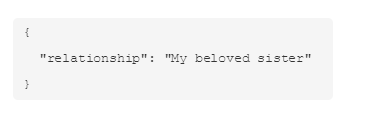
\includegraphics[width=0.7\textwidth]{image/quan_he_thuoc_tin.PNG}
\caption{\label{fig:relationshipsprop} Quan hệ LIKES từ mèo Stormy đối với Pusheen}
\end{figure}

% chuong 3
\section{Cypher}

Cypher là ngôn ngữ truy vấn cho cơ sở dữ liệu đồ thị. Một câu truy vấn có cấu trúc như hình \ref{fig:cypher}.

\begin{figure}[h]
\centering
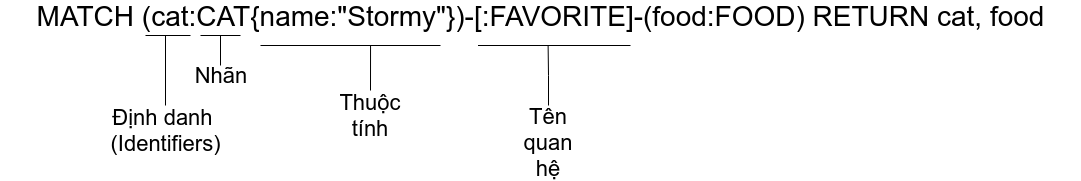
\includegraphics[width=0.8\textwidth]{image/chap2cypher.png}
\caption{\label{fig:cypher} Cấu trúc một Cypher đơn giản }
\end{figure}

Một Cypher bao gồm nhiều vế 
\begin{itemize}
\item MATCH 
\item CREATE 
\item RETURN
\item WHERE
\item MERGE
\item DELETE
\item SET
\item FOREACH 
\item UNION
\item WITH 
\item START
\end{itemize}

\subsection{Triết lý của Cypher}
\label{sec:cypherpil}
Cypher được thiết kế để mọi người, bao gồm người lập trình, chuyên viên cơ sở dữ liệu, và các nghiệp vụ liên quan có thể đọc và hiểu dễ dàng. Cypher sử dụng sơ đồ (vẽ ASCII) để vẽ đồ thị

\begin{figure}[h]
\centering
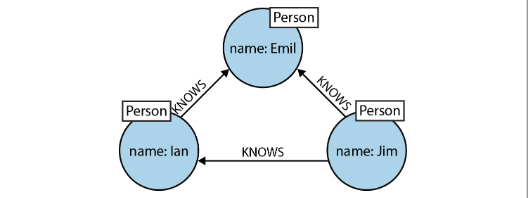
\includegraphics[width=0.8\textwidth]{image/chap3graphdiagram.png}
\caption{\label{fig:graphdiagram} Đồ thị}
\end{figure}

Đồ thị như hình \ref{fig:graphdiagram} được biểu diễn như sau: 

\begin{lstlisting}[caption={Cypher}, label={lst:cypherjim1}, language=SQL]
(emil)<-[:KNOWS]-(jim)-[:KNOWS]->(ian)-[:KNOWS]->(emil) 
\end{lstlisting}

% (emil)<-[:KNOWS]-(jim)-[:KNOWS]->(ian)-[:KNOWS]->(emil) 

Cypher ở listing \ref{lst:cypherjim1} thể hiện "đường đi" từ jim tới hai nút tên là ian và emil. Nút ian cũng nối tới nút emil. ian, jim và emil là định danh (identifier). Định danh giúp ta chỉ tới một nút nhiều hơn một lần khi ta định nghĩa một đồ thị. 

\begin{lstlisting}[caption={Cypher với thuộc tính}, label={lst:cypherjim2}, language=SQL]
(emil:Person {name:'Emil'})
<-[:KNOWS]-(jim:Person {name:'Jim'})
-[:KNOWS]->(ian:Person {name:'Ian'})
-[:KNOWS]->(emil) 
\end{lstlisting}

Listing \ref{lst:cypherjim2} cùng định nghĩa một đồ thị ở hình \ref{fig:graphdiagram} nhưng có thêm thuộc tính. Định danh emil gắn với nút có nhãn là Person và có thuộc tính name có giá trị là Emil. 

\subsection{Tìm với MATCH}

MATCH là một trong những vế quan trọng của Cypher. Về MATCH sử dụng hình vẽ ASCII để biểu diễn đồ thị (như đẵ trình bày ở mục \ref{sec:cypherpil}.

\begin{itemize}
\item Ta biểu diễn nút (node) trong ngoặc tròn. Ví dụ: (jim:Person {name:'Jim'})
\item Ta biểu diễn quan hệ (relationship) bằng dấu hai dấu gạch ngang với dấu lớn hơn, bé hơn (--> và <--). Dấu lớn hơn, bé hơn thể hiện hướng quan hệ. Giữa hai dấu gạch, ta biểu diển tên quan định danh (nếu có) và tên quan hệ trong dấu ngoặc vuông, ngăn cách bằng dấu hai chấm. Ví dụ:  <-[:KNOWS]-
\end{itemize}

\begin{lstlisting}[caption={Cypher query từ người tên Jim}, label={lst:cypherjim3}]
MATCH (a:Person{name:'Jim'})-[:KNOWS]->(b)-[:KNOWS]->(c),
(a)-[:KNOWS]->(c) 
RETURN b, c 
\end{lstlisting}

\begin{lstlisting}[caption={Cypher query từ người tên Jim sử dụng WHERE}, label={lst:cypherjim4}]
MATCH (a:Person{name:'Jim'})-[:KNOWS]->(b)-[:KNOWS]->(c),
(a)-[:KNOWS]->(c) 
WHERE a.name = 'Jim'
RETURN b, c 
\end{lstlisting}

Listing \ref{lst:cypherjim3} và listing \ref{lst:cypherjim4} dùng để truy vấn mối quan hệ từ nút có name giá trị Jim. Nhưng ở listing \ref{lst:cypherjim4} thay vì gắn thuộc tính vào vế MATCH thì ta dùng vế WHERE để tìm nút theo thuộc tính.   

\subsection{RETURN}
Vế RETURN trả về những nút, hoặc quan hệ được ràng buộc vào những định danh được liệt kê trong vế RETURN. Listing \ref{lst:cypherjim3} trả về nút có định danh b và nút có định danh c. 

\subsection{Tạo thêm nút và quan hệ với CREATE}
Vế CREATE kèm theo hình vẽ ASCII để tạo sơ đồ theo hình vẽ ấy. Listing \ref{lst:create1} tạo mới một nút có nhãn là CAT và gán thuộc tính name có giá trị là Pusheen. Listing \ref{lst:create1} tạo hai nút và quan hệ từ nút có thuộc tính name là Pusheen qua nút có thuộc tính name là Stormy. Ở vế CREATE, mối quan hệ luôn luôn có hướng vì Neo4j chỉ cho phép quan hệ có hướng.

\begin{lstlisting}[caption={Cypher tạo mới nút}, label={lst:create1}]
CREATE (cat:CAT{name:"Pusheen"})
\end{lstlisting}

\begin{lstlisting}[caption={Cypher tạo mới hai nút và quan hệ giữa hai nút}, label={lst:create2}]
CREATE (:CAT{name:"Pusheen"})-[:LIKES]->(:CAT{name:"Stormy"})
\end{lstlisting}

Ngoài ra, có thể kết hợp với vế MATCH để tạo thêm đồ thị có liên kết với một phần đồ thị đã có trước đó. 
Ở listing \ref{lst:create3}, vế MATCH nút CAT có thuộc tính name mang giá trị Pusheen và gắn định danh là a. Sau đó, vế CREATE tạo nút CAT có thuộc tính name là Stormy, và tạo quan hệ hướng từ nút định danh a sang nút mới tạo 

\begin{lstlisting}[caption={Cypher tạo nút và quan hệ nối với nút có sẵn}, label={lst:create3}]
MATCH (a:CAT{name:"Pusheen"})
CREATE (a)-[:LIKES]->(:CAT{name:"Stormy"})
\end{lstlisting}


\subsection{Một vài vế khác}

MERGE: đảm bảo trong đồ thì tồn tại cái sơ đồ được cung cấp bằng cách tái sử dụng nút và quan hệ thỏa các điều kiện cho trước, hoặc tạo các nút và quan hệ mới. 

DELETE: xóa nút, quan hệ, thuộc tính. (Ví dụ listing \ref{lst:cypherdelete})
\begin{lstlisting}[caption={Cypher xóa}, label={lst:cypherdelete}]
MATCH (a:CAT{name:"Tom"})
DELETE a
\end{lstlisting}

SET: thêm, chỉnh sửa thuộc tính (ví dụ listing \ref{lst:cypherset})
\begin{lstlisting}[caption={Cypher sửa}, label={lst:cypherset}]
MATCH (a:CAT{name:"Tom"})
SET a.name="Thomas", a.age=1
\end{lstlisting}

UNION: gộp kết quả của hai hoặc nhiều truy vấn 

START: Chọn một hoặc một số điểm bắt đầu (nút hoặc quan hệ). START không được phát triển nữa. Ta nên dùng MATCH 

\section{Xây dựng ứng dung dữ liệu đồ thị}

\subsection{Đặc tả mô hình dữ liệu theo nhu cầu của ứng dụng}

Câu hỏi mà ta cần hỏi dữ liệu giúp ta xác định thực thể và mối quan hệ. Câu chuyện người dùng (user-stories) cho cái nhìn trực quan, tập trung vào nhu cầu người dùng cuả ứng dụng. 

Ví dụ: 

"\textbf{LÀ} một đọc giả, \textbf{TÔI MUỐN} biết những cuốn sách yêu thích của các đọc giả khác cùng thích những cuốn sách giống tôi \textbf{ĐỂ} tôi có thể tìm thêm sách để đọc"

Qua câu chuyện người dùng này, vế \textbf{LÀ} giúp ta xác định thành phần của đồ thị, bao gồm 

\begin{itemize}
\item Nút: sách  
\item Nút: đọc giả 
\item Quan hệ: thích  
\end{itemize}

Vế \textbf{TÔI MUỐN} đặt câu hỏi: Sách nào mà những đọc giả cùng đọc sách giống tôi thích. Vế này thể hiện quan hệ thích  và các thực thể sách, đọc giả khác.

\begin{figure}[h]
\centering
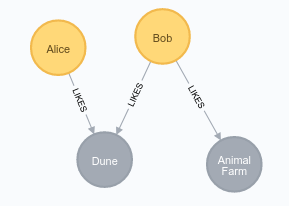
\includegraphics[width=0.8\textwidth]{image/bookfull.png}
\caption{\label{fig:graphbook} Đồ thị sách}
\end{figure}

Ta có đồ thị như hình \ref{fig:graphbook}. Giả sử người dùng là Alice, Alice muốn tìm xem những người thích cuốn sách Dune sẽ thích cuốn nào. Ta sẽ dùng câu truy vấn 

\begin{lstlisting}[caption={Cypher tìm người thích đọc sách tên Dune}, label={lst:cypherdune}]
MATCH (:READER {name:'Alice'})-[:LIKES]->(:BOOK {name:'Dune'})<-[:LIKES]-(:READER)-[:LIKES]->(books:BOOK) RETURN books
\end{lstlisting}

\subsection{Nút biểu diễn vật thể, quan hệ biểu diễn cấu trúc}

Một số quy tắc khi nào dùng nút, khi nào dùng quan hệ

\begin{itemize}
\item Nút thể hiện thực thể, nó là cái vật gì đó trong lĩnh vực mà ta quan tâm. Vật đó có thể gán nhãn và nhóm 
\item Quan hệ thể hiện sự liên kết giữa các thực thể và xây dựng nên bối cảnh về mặc ngữ nghĩa cho mỗi thực thể, cấu thành miền ta quan tâm
\item Dùng hướng của quan hệ để làm rõ mối liên kết ngữ nghĩa. Đối với các quan hệ vô hướng, ta không nên tạo 2 quan hệ mà chỉ cần mặc kệ hướng của quan hệ trong câu truy vấn 
\item Thuộc tính của nút là thuộc tính của thực thể, thêm những thông tin hệ thống như mốc thời gian, phiên bản 
\item Sử dụng thuộc tính của quan hệ để thể hiện hệ số, mức quan trọng, chất lượng của quan hệ, và thêm nhưng thông tin hệ thống như mốc thời gian, phiên bản 
\end{itemize}




\subsection{Quan hệ chung với quan hệ chuyên môn hóa}

\subsection{}


%%%%%%%%%%%%%%%%%%%%%%%%%%%%%%%%%%%%%%%%%%%%%%%%%%%%
% Comments can be added to the margins of the document using the \todo{Here's a comment in the margin!} todo command, as shown in the example on the right. You can also add inline comments too:

% \todo[inline, color=green!40]{This is an inline comment.}



\subsection{Tables and Figures}

Use the table and tabular commands for basic tables --- see Table~\ref{tab:widgets}, for example. You can upload a figure (JPEG, PNG or PDF) using the files menu. To include it in your document, use the includegraphics command as in the code for Figure~\ref{fig:frog} below.

% % Commands to include a figure:
% \begin{figure}
% \centering
% 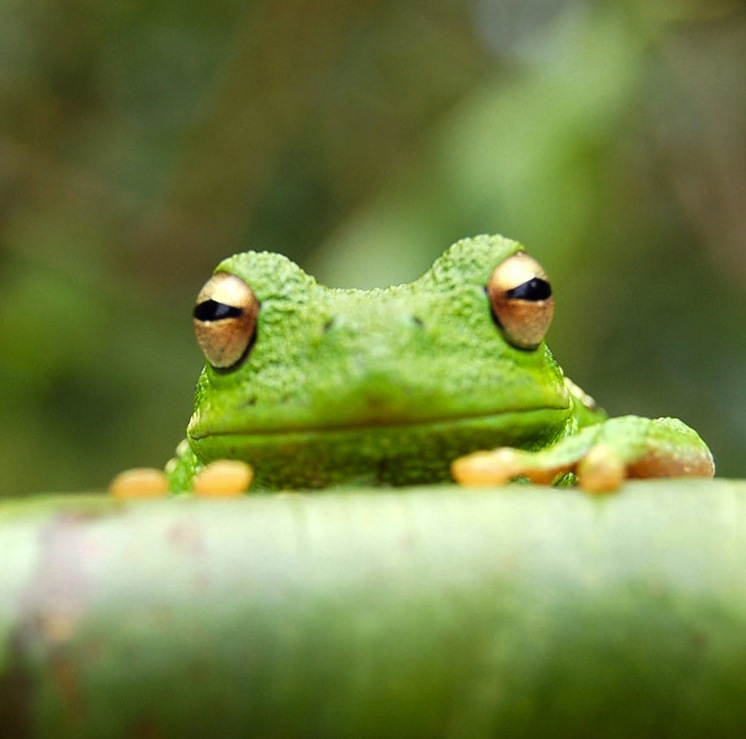
\includegraphics[width=0.5\textwidth]{frog.jpg}
% \caption{\label{fig:frog}This is a figure caption.}
% \end{figure}

% \begin{table}
% \centering
% \begin{tabular}{l|r}
% Item & Quantity \\\hline
% Widgets & 42 \\
% Gadgets & 13
% \end{tabular}
% \caption{\label{tab:widgets}An example table.}
% \end{table}

\subsection{Mathematics}

\LaTeX{} is great at typesetting mathematics. Let $X_1, X_2, \ldots, X_n$ be a sequence of independent and identically distributed random variables with $\text{E}[X_i] = \mu$ and $\text{Var}[X_i] = \sigma^2 < \infty$, and let
$$S_n = \frac{X_1 + X_2 + \cdots + X_n}{n}
      = \frac{1}{n}\sum_{i}^{n} X_i$$
denote their mean. Then as $n$ approaches infinity, the random variables $\sqrt{n}(S_n - \mu)$ converge in distribution to a normal $\mathcal{N}(0, \sigma^2)$.

\subsection{Lists}

You can make lists with automatic numbering \dots

\begin{enumerate}
\item Like this,
\item and like this.
\end{enumerate}
\dots or bullet points \dots
\begin{itemize}
\item Like this,
\item and like this.
\end{itemize}

We hope you find write\LaTeX\ useful, and please let us know if you have any feedback using the help menu above.

\end{document}